\documentclass{beamer}
\usetheme{Boadilla}
\usepackage[ngerman]{babel}
\usepackage[utf8]{inputenc}
\usepackage[T1]{fontenc}
\usepackage{lmodern}
\usepackage{hyperref}
\usepackage{listings} 
\usepackage{graphicx}
\usepackage{pgf}
\usepackage{color}
\definecolor{ex_green_titel}{RGB}{204,230,204}
\definecolor{ex_green}{RGB}{230,243,230}
\definecolor{light-gray}{gray}{0.95}

\begin{document}
\lstset{ 						%
language=bash,                % the language of the code
basicstyle=\footnotesize,       % the size of the fonts that are used for the code
%numbers=right,                   % where to put the line-numbers
n%umberstyle=\footnotesize,      % the size of the fonts that are used for the line-numbers
%stepnumber=2,                   % the step between two line-numbers. If it's 1, each line 
                                % will be numbered
numbersep=-10pt,                  % how far the line-numbers are from the code
backgroundcolor=\color{light-gray},  % choose the background color. You must add \usepackage{color}
showspaces=false,               % show spaces adding particular underscores
showstringspaces=false,         % underline spaces within strings
showtabs=false,                 % show tabs within strings adding particular underscores
frame=single,                   % adds a frame around the code
tabsize=2,                      % sets default tabsize to 2 spaces
captionpos=b,                   % sets the caption-position to bottom
breaklines=true,                % sets automatic line breaking
breakatwhitespace=false,        % sets if automatic breaks should only happen at whitespace
%title=\lstname,                 % show the filename of files included with \lstinputlisting;
                                % also try caption instead of title
escapeinside={\%*}{*)},         % if you want to add a comment within your code
morekeywords={*,...}            % if you want to add more keywords to the set
}

\title{Eine Einführung in Versionverwaltungsysteme}   
\subtitle{Wissenswertes für GIT-Anwender}
\titlegraphic{
\includegraphics[width=2cm,height=2cm]{erlangen}}
\author[Bernd Wunder]{bernd.wunder@leb.eei.uni-erlangen.de} 
\institute[LEB -- TF Uni Erlangen]{Lehrstuhl für Elektronische Bauelemente\\ Friedrich-Alexander-Universität Erlangen-Nürnberg}
\date{\today}
\logo{
\includegraphics[scale=0.08]{erlangen}}

\begin{frame}
\titlepage
\end{frame}

\begin{frame}
\frametitle{Inhaltsverzeichnis}\tableofcontents
\end{frame}

%--- Einführung ---
\section{Einführung} 

%--- Was ist ein Versionsverwaltungsystem ---
\subsection{Was ist ein Versionsverwaltungsystem}

%--- Was ist ein Versionsverwaltungsystem ---
\begin{frame}\frametitle{Was ist ein Versionsverwaltungsystem} 
\begin{quote}
Eine Versionsverwaltung ist ein System, das zur Erfassung von Änderungen an Dokumenten oder Dateien verwendet wird. Alle Versionen werden in einem Archiv mit Zeitstempel und Benutzerkennung gesichert und können später wiederhergestellt werden.
\footnote{Quelle: \href{http://de.wikipedia.org/wiki/Versionsverwaltung}{Wikipedia}}
\end{quote} 

Aufgaben
\begin{itemize}
\item  Protokollierungen der Änderungen
\item  Wiederherstellung von alten Ständen 
\item  Archivierung der einzelnen Stände eines Projektes
\item  Kooperative Entwicklung (Entwicklungsteams)
\item  gleichzeitige Entwicklung mehrerer Entwicklungszweige (branches)
\end{itemize} 
\end{frame}

%----- Warum Versionsverwaltung -----
\subsection{Warum Versionsverwaltung}

%--- Warum Versionsverwaltung ---
\begin{frame}\frametitle{Warum Versionsverwaltung}
\begin{columns}
        \column{.55\textwidth}
                \pgfimage[width=\textwidth]{Bilder/chaosschreibtisch}
        \column{.45\textwidth}
                \begin{enumerate}
                \item viele gleichzeitige laufende Projekte / Features (z.B. Sicherheitsupdates, neue Funktionstests, verschiedene Versionen)
                \item Um des Chaos Herr zu werden
                \end{enumerate}
\end{columns}
\end{frame}

%--- Warum Versionsverwaltung ---
\begin{frame}\frametitle{Warum Versionsverwaltung}
\begin{columns}
        \column{.55\textwidth}
                \pgfimage[width=\textwidth]{Bilder/schreibtisch}
        \column{.45\textwidth}
                \begin{enumerate}
                \item viele gleichzeitige laufende Projekte / Features (z.B. Sicherheitsupdates, neue  Funktionstests, verschiedene Versionen)
                \item Um des Chaos Herr zu werden
                \item Überblick über die gesamte Entwicklung behalten
                \item kolaboratives Arbeiten in einem Team
                \end{enumerate}
\end{columns}
\end{frame}

%----- Übersicht über Versionsverwaltungsysteme -----
\subsection{Übersicht über Versionsverwaltungssysteme}

%--- Übersicht über Versionsverwaltungsysteme ---
\begin{frame}\frametitle{Übersicht über Versionssverwaltungsysteme} 
engl. Bezeichnungen: \textit{Version Control System (VCS)}, \textit{Software Configuration Management (SCM)}, \textit{Revision Control System (RCS)}
\vspace*{0.15cm}
\textbf{unvollständige Übersicht einiger VCSe:}
\begin{block}{Revision Control System (RCS)}
	\begin{tabular}{l c}
Entwicklung: & 1980 bis 2004  \\  
Einteilung: & zentrales, dateibasiertes VCS \\ 
Probleme: & Binärdateien, Verzeichnisse, locks, merge, \\
          & keine Atomic commits, keine Metadaten, umbenennen  \\
Lizenz: & GPL2 \\
Betriebsysteme: & UNIX, WIN95 \\

\end{tabular} 

\vspace*{0.3cm}
Entwickelt für die Versionsverwaltung von Text-Dateien auf einem Computer!
RCS ist im Wesentlichen mit dem ersten VCS, dem \textit{Source Code Control System (SCCS)}, vergleichbar.
\end{block}
\end{frame}

%--- Versionsverwaltungsysteme ---
\begin{frame}\frametitle{Versionsverwaltungsysteme} 
\begin{block}{Concurrent Versions System (CVS)}
	\begin{tabular}{l c}
basierend auf: & RCP (nutzt gleiches Speicherformat) \\ 
Entwicklung: & 1989 bis 2008  \\  
Einteilung: & zentrales VCS \\ 
Probleme: & Binärdateien, Verzeichnisse, locks, merge, \\
          & keine Atomic commits, keine Metadaten, umbenennen  \\
Lizenz: & GPL2 \\
Betriebsysteme: & UNIX, WINDOWS, Mac OS X \\
\end{tabular} 

\vspace*{0.3cm}
CVS wird nicht mehr aktiv weiterentwickelt. Die offizielle Webseite wird nicht mehr weiter betreut. \footnote{Quelle: \href{http://de.wikipedia.org/wiki/Concurrent_Versions_System}{Wikipedia}}
\end{block}
\end{frame}

%--- Versionsverwaltungsysteme ---
\begin{frame}\frametitle{Versionsverwaltungsysteme} 
\begin{block}{Subversion (SVN)}
	\begin{tabular}{l c}
basierend auf: & CVS (Nachfolger) \\ 
Entwicklung: & seit 2000  \\  
 & Ziele CVS Probleme (siehe oben) zu beseitigen \\
Einteilung: & zentrales VCS \\ 
Probleme: & Binärdateien, Verzeichnisse, locks, merge \\
Lizenz: & Apache License \\
Betriebsysteme: & UNIX, WINDOWS, Mac OS X \\
\end{tabular} 
\begin{quote}
Subversion versteht sich als Weiterentwicklung von CVS und entstand als Reaktion auf weit verbreitete Kritik an CVS. In der Bedienung der Kommandozeilenversion ist es sehr ähnlich gehalten.  \footnote{Quelle: \href{http://de.wikipedia.org/wiki/Subversion_\%28Software\%29}{Wikipedia}}
\end{quote}
\end{block}
\end{frame}

%--- Vergleich einiger Versionsverwaltungsysteme ---
\begin{frame}\frametitle{Vergleich\footnote{Quelle: \href{http://better-scm.shlomifish.org/comparison/comparison.html}{Version Control System Comparison}} einiger Versionsverwaltungsysteme }
\begin{exampleblock}{Vergleich | CVS,SVN,GIT,Mercurial}
	\begin{tabular}{l|c c c c}
	\hline
		\textbf{Operation} & \textbf{CVS} & \textbf{SVN} & \textbf{GIT} & \textbf{Mercurial} \\
	\hline
	\hline
		Atomic Commits: & Nein & Ja & Ja & Ja \\
	\hline
		Umbenennen/Verschieben von\\
		Dateien und Verzeichnissen: & Nein & Ja & Ja & Ja \\
	\hline
		Intelligente Merges \\ 
		nach Umbenungen/Verschiebungen: & Nein & Nein & Nein & Ja \\
	\hline
		Verzeichnisse/Dateien mit History \\
		im Repository kopieren: & Nein & Ja & Nein & Ja \\
	\hline		
		Remote Kopie in lokales Verzeichnis: & Nein & Nein & Ja & Ja \\
	\hline		
		Änderungen an andere \\
		Repository weitergeben: & Nein & Nein & Ja & Ja \\		
	\hline		
		Changesets Support & Nein & teilw. & Ja & Ja \\ 		
	\hline
	\hline
\end{tabular} 
\end{exampleblock}
\end{frame}

%--- Warum Git? ---
\begin{frame}\frametitle{Warum Git?}
\begin{description}
\item[Speed] Schnellstes mir bekannte Versionsverwaltungssystem 
\item[Branch] sehr einfach Zweige (Branch) zu erstellen und zusammenzuführen!
\item[Lokal] alle Informationen sind lokal gespeichert, keine Netzwerkverbindung notwendig!
\item[Speicher] sehr geringer Speicherverbrauch durch Kompression
\end{description}

\begin{figure}
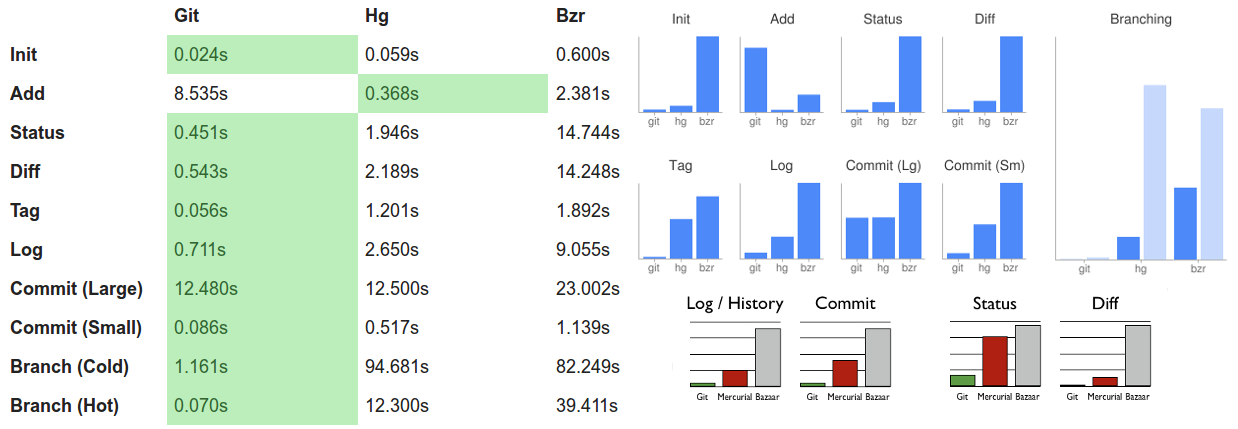
\includegraphics[scale=0.25]{Bilder/speed2} 
\caption{Geschwindigkeitsvergleich von Git, Mercuial und Baszar}
\end{figure}
\end{frame}

%--- Warum Git? ---
\begin{frame}\frametitle{Warum Git?}
\begin{description}
\item[Protokoll] http, https, ssh, git, ...
\item[Kooperativ] gute Zusammenarbeit mit anderen Versionsverwaltungssystemen. Z.B. mit SVN oder CVS
\item[Stabil] sehr aktives Projekt mit vielen hundert Entwicklern
\item[tested] Protokiv im Einsatz bei Linux-Kernel (>1000 Entwickler)
\end{description}

\begin{figure}
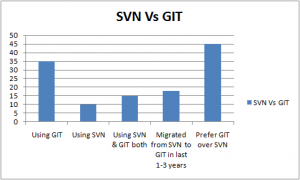
\includegraphics[scale=0.5]{Bilder/svnvsgit1} 
\caption{Geschwindigkeitsvergleich von Git, Mercuial und Baszar}
\end{figure}
\end{frame}

%--- Warum Git? ---
\begin{frame}\frametitle{Wer nutzt Git?}
Viele Open Source Projekte setzen bereits Git ein:

\begin{columns}
        \column{.5\textwidth}
                \begin{itemize}                
					\item Linux Kernel
					\item Git
					\item Android (Google's Handy OS) 
					\item CakePHP (PHP Framework) 
					\item Debian - Linux Distribution
					\item Drupal - CMS System
					\item Typo3 - CMS System
					\item Perl
					\item Ruby on Rails
	                \item VLC
                \end{itemize}
        \column{.5\textwidth}
                \begin{itemize}
                \item PostgreSQL
                \item KDE
                \item Fluxbox
                \item X.Org
                \item GCC (Gnu Compiler Collection)
                \item JQuery (JavaScript library) 
                \item Qt (Cross-platform graphic toolkit)
                \item Eclipse
                \item Gnome
                \item ...
                \end{itemize}
\end{columns}

\end{frame}

%--- Grundbegriffe ---
\subsection{Grundbegriffe}

%--- Grundbegriffe (GIT) ---
\begin{frame}\frametitle{Grundbegriffe}
\begin{block}{Repository}
Datenbank in dem jeder Dateistand eines Projektes über die Zeit hinweg gespeichert ist.
\end{block}
\begin{block}{Working Tree}
Arbeitsverzeichnis in dem die Modifikationen durchgeführt werden.
\end{block}
\begin{block}{Commit}
beinhaltet alle Veränderungen bzw. spiegelt den aktuellen Zustand der in das VCS aufgenommen werden soll wieder. Enthält neben den Änderungen zusätzliche Metadaten (Commit Message, Autor, Datum, Signatur, ...)
\end{block}
\begin{block}{HEAD}
zeigt auf die neueste Version \textit{Kopf} im aktuellen Zweig (Branch)

Achtung: Unterschide zwischen GIT und SVN,CVS
\end{block}
\end{frame}

%--- Grundbegriffe (GIT) ---
\begin{frame}\frametitle{Grundbegriffe}
\begin{block}{Secure Hash Algorithm (SHA-1)}
ist eine eindeutige, 160 Bit (40 hexadezimale Zeichen) lange Prüfsumme für beliebige digitale Informationen.
\end{block}
\begin{exampleblock}{Beispiel:}
mit dem GNU/Linux Programm \textit{sha1sum} wird die Prüfsumme für den Text \textit{"'Isabella und Lilly Wunder"'} berechnet werden:
\lstinputlisting{bash.txt}
\end{exampleblock}
\end{frame}

%--- Grundbegriffe (GIT) ---
\begin{frame}\frametitle{Grundbegriffe (GIT)}
\begin{block}{\textit{Branch}}
bezeichnet einen parallelen Entwicklungszweig. Der Hauptzweig in einem Versionsverwaltungssystem hat meistens einen speziellen Namen. ( z.B in SVN->\textit{trunk} und in GIT->\textit{master})
\end{block}
\begin{block}{Objektmodell}
Git-Objekte (blob, tree, commit, tag) sind in einer Objektdatenbank gespeichert und über SHA1-Summen identifizierbar. Die History eines Repository lässt sich als Graph von Objekten modellieren.
\end{block}
\begin{block}{\textit{Index}}
Der \textit{Index} ist ein lokaler Zwischenspeicher. Alle Änderungen werden zuerst in den index geschrieben. Anschießend wird der Index durch einen \textit{commit} in das Repository eingecheckt. 
\end{block}
\end{frame}

%--- Grundbegriffe (GIT) ---
\begin{frame}\frametitle{Grundbegriffe (GIT)}
\begin{block}{\textit{Clone}}
ist eine Kopie eines Repositories mit der gesamten History der Entwicklung.
\end{block}
\begin{block}{\textit{Tag}}
Ein Tag ist ein symbolischer Name für schwer zu merkende SHA-1 Summen. So können spezielle \textit{Commit} einen Namen, also ein \textit{Tag} erhalten. 
\end{block}
\end{frame}

%--- History als Graph: Von Branches, Merges und Tags ---
\begin{frame}\frametitle{History als Graph: Von Branches, Merges und Tags}
\begin{description}
\item[Branch] Parralle Entwicklung in Teams erfordert oft mehrere Zweige
\item[Tag] Name für eine bestimmte Version 
\item[Merge] Führt den Parallelen Zweig in den Hauptzweig zurück
\item[Trunk] Name in SVN für den Hauptentwicklungszweig
\end{description}

\begin{figure}
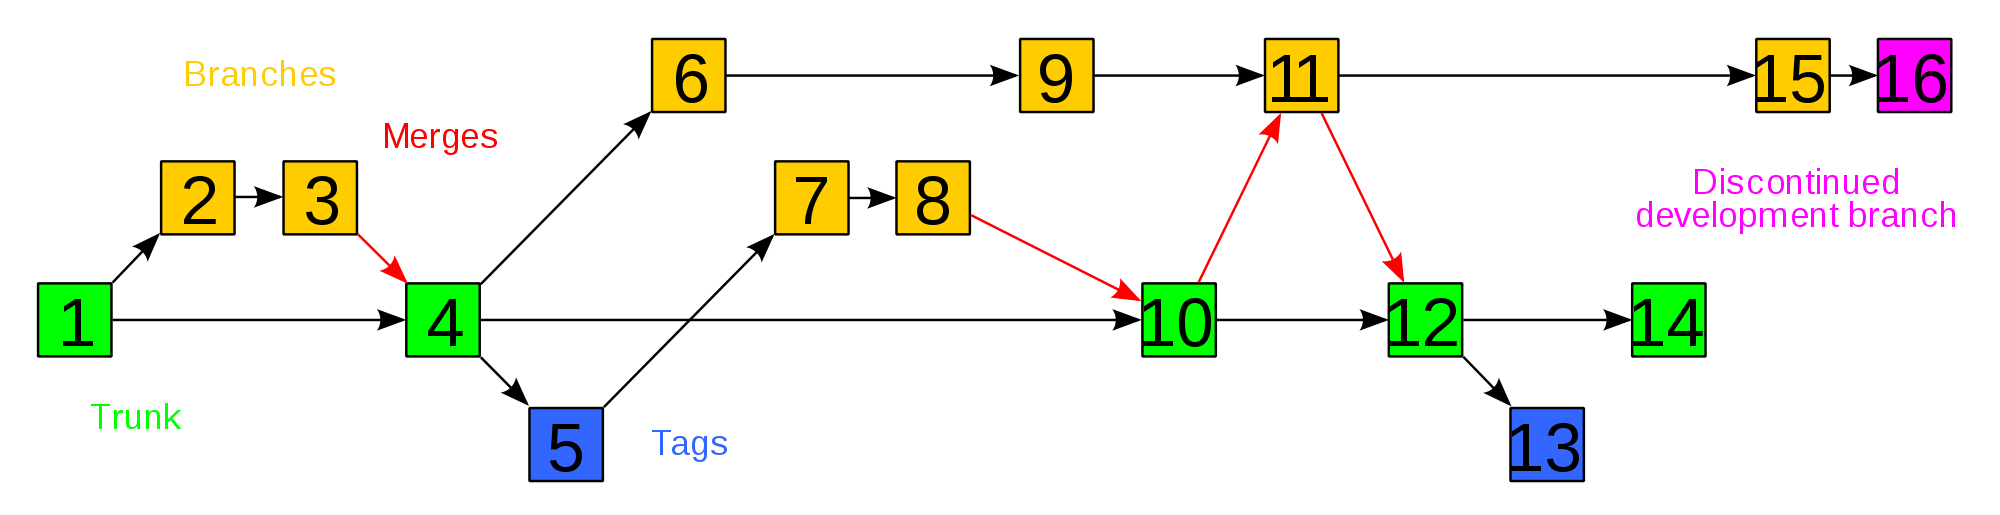
\includegraphics[scale=0.15]{2000px-Subversion_project_visualization} 
\caption{Branches, Merges und Tags \footnote{Quelle: \href{http://en.wikipedia.org/wiki/File:Subversion_project_visualization.svg}{Wikipedia}}}
\end{figure}
\end{frame}

%----- Lokale, zentrale und verteilte Versionsverwaltungssysteme -----
\section{Lokale, zentrale und verteilte Versionsverwaltungssysteme} 

%----- Branches, Merges und Tags -----
\begin{frame}\frametitle{Lokale, zentrale und verteilte Versionsverwaltungssysteme}
\begin{description}
\item[lokal] rcs: einfache Ergänzung des Dateisystems.
\item[zentral] Subversion (SVN), CVS: Kommunikation nur über zentralen Server.
\item[verteilt] Git, Baszar, Merkurial: Kommunikation beliebig.

\end{description}

\begin{figure}
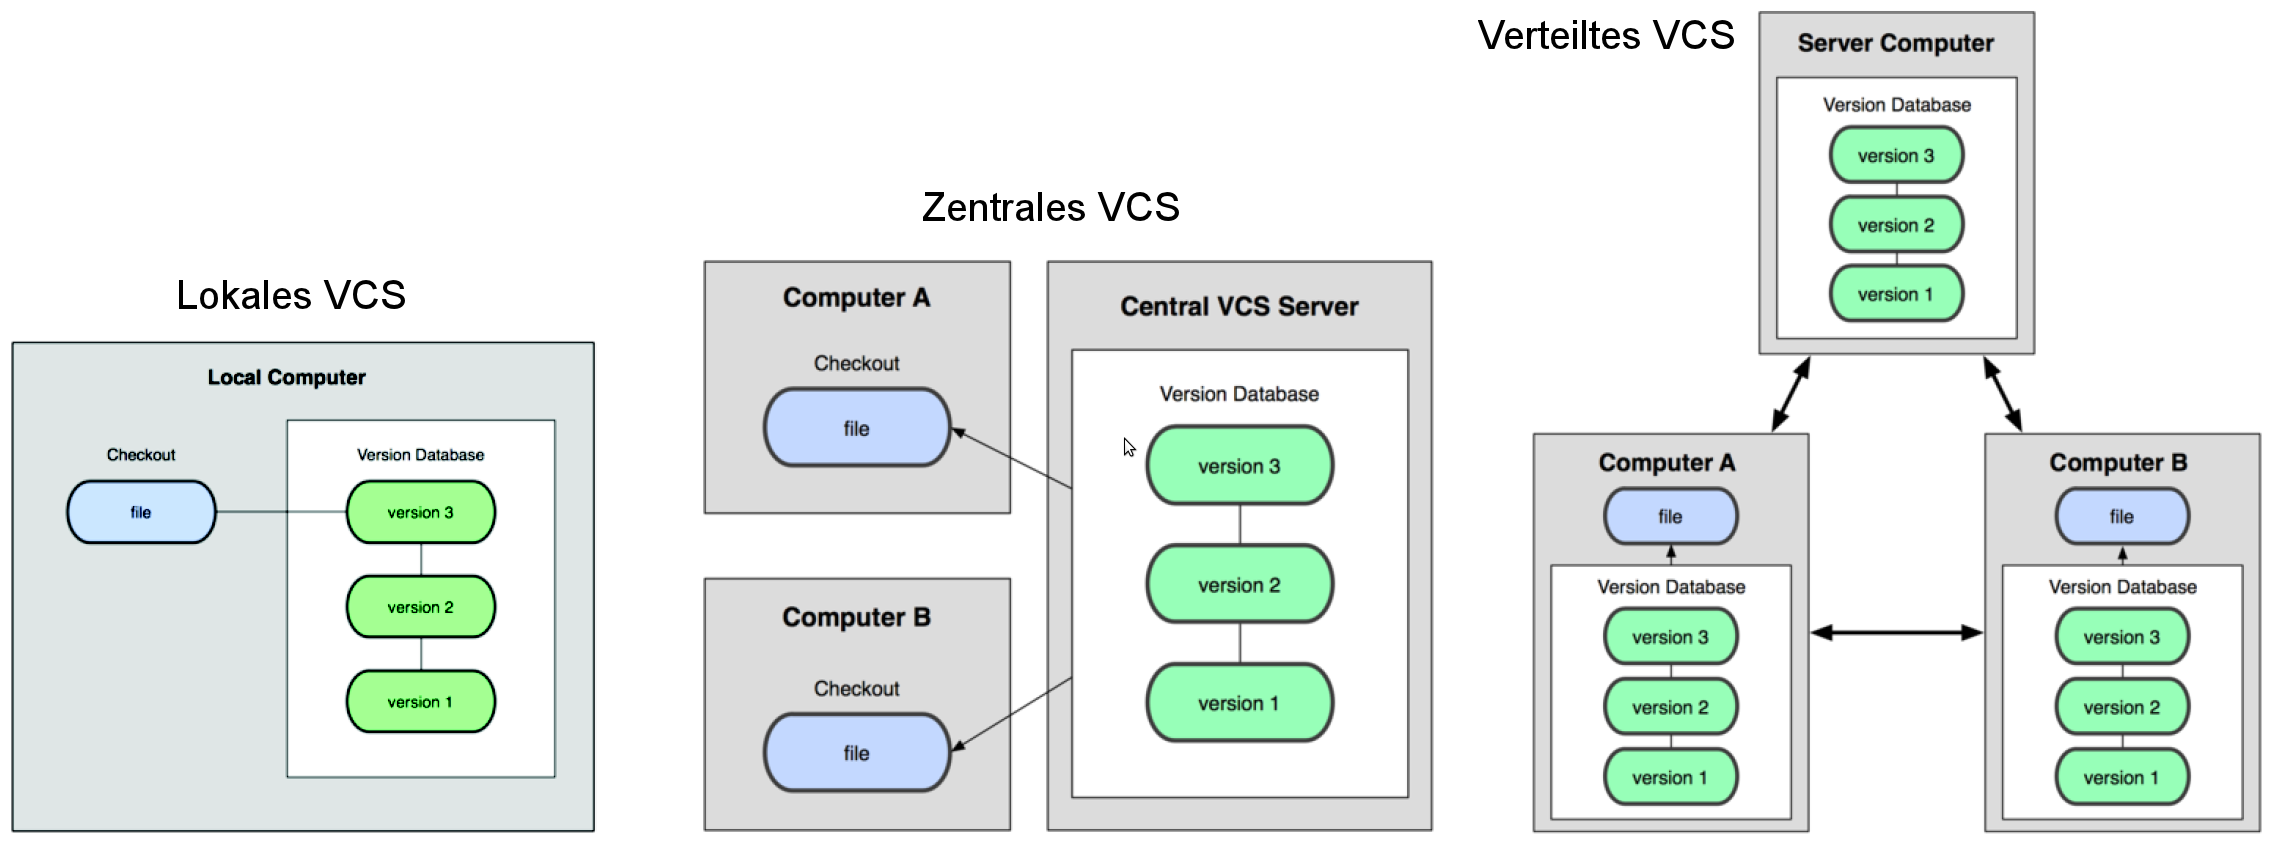
\includegraphics[scale=.15]{Bilder/VCSArten}
\caption{Unterschiedliche Arten von Versionsverwaltungssystemen
 \footnote{Quelle: \href{http://progit.org/}{Pro Git - Scott Chacon}}}
\end{figure}
\end{frame}

%----- Tools -----
\section{Tools}

%----- gitk -----
\subsection{gitk}

%--- Repository Tool: gitk ---
\begin{frame}\frametitle{Repository Tool: \textit{gitk}}
\begin{block}{\textit{gitk}}
In Tcl programmiertes grafisches Frontend zur Anzeige des Repositories. Ist im Git Standard Umfang enthalten und somit \textbf{immer} vorhanden. Ermöglicht einen schnellen Überblick über die History, Commits, Diffs, Tags und die Struktur des Repositories. 
\end{block}

\begin{figure}
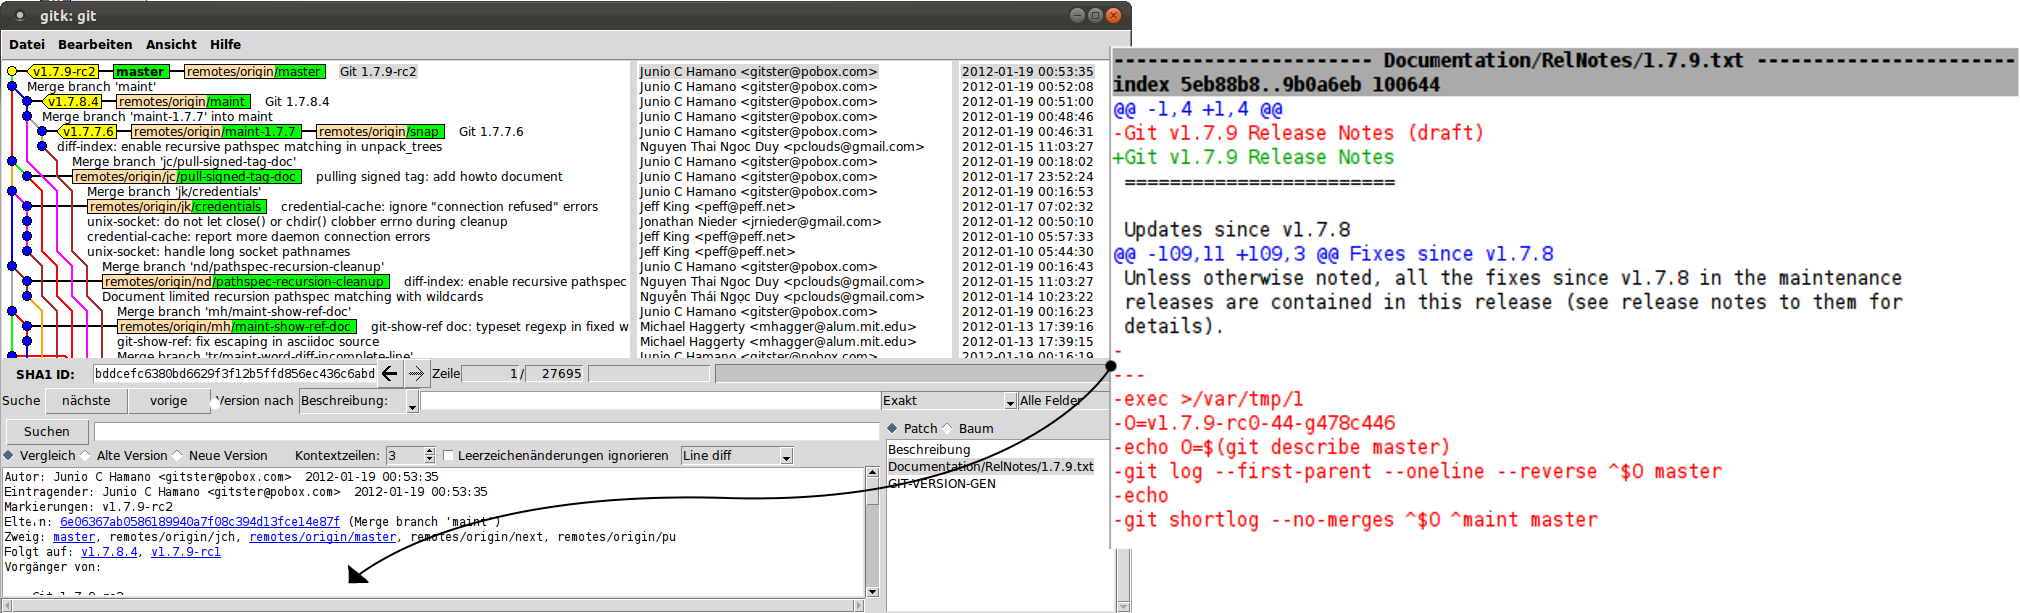
\includegraphics[scale=0.7]{Bilder/gitk} 
\caption{\textit{gitk}: einfach, übersichtlich und immer da!}
\end{figure}
\end{frame}

\subsection{git-gui}
\begin{frame}\frametitle{Commit Tool: \textit{git-gui}}
\begin{block}{\textit{git-gui}}
Einfaches grafisches Programm um Änderungen bereitzustellen und einen Commits zu erstellen. 
\end{block}

\begin{figure}
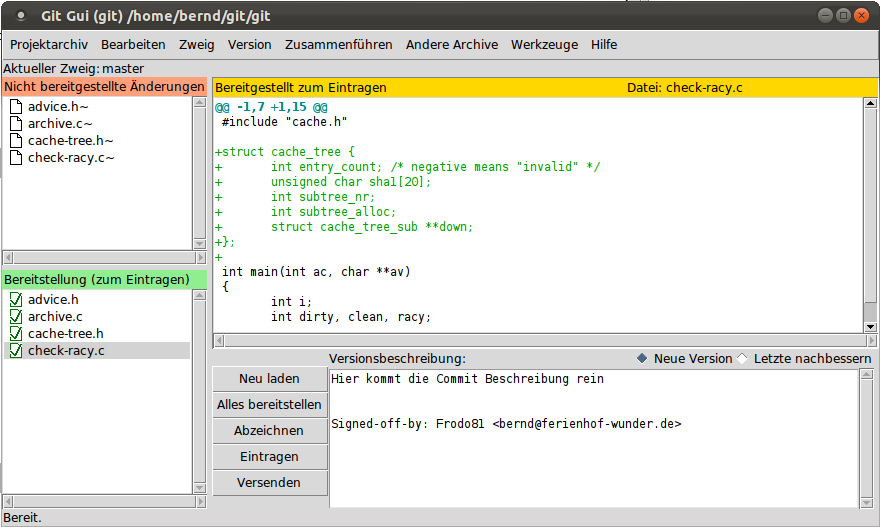
\includegraphics[scale=1.1]{Bilder/git_gui} 
\caption{\textit{git-gui}: Frontend für die Erstellung eines Commits. Ist wie \textit{gitk} im Standardumfang enthalten.}
\end{figure}
\end{frame}

%----- Diff-Tools -----
\subsection{Diff-Tools}

%--- Diff-Tool: meld ---
\begin{frame}\frametitle{Diff-Tool: meld}
%\begin{block}{gitk}
%Diffs betrachten und mergen (zusammenführen) von Änderungen und Konflikten.
%\end{block}

\begin{figure}
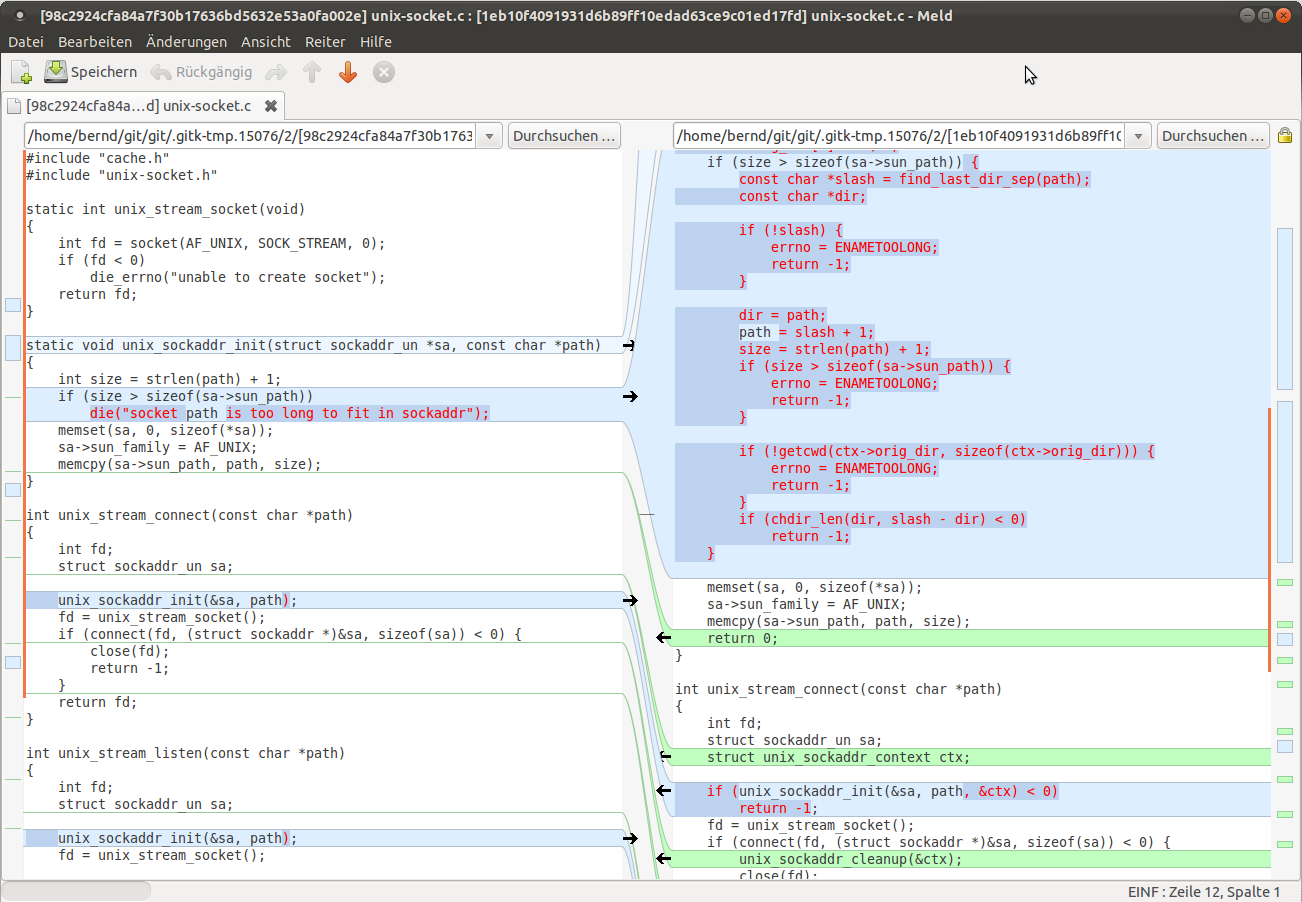
\includegraphics[scale=0.9]{Bilder/meld} 
\caption{\textit{meld}: einfach, übersichtlich und immer da!}
\end{figure}
\end{frame}


%----- Befehle -----
\section{Befehle}

%--- Befehle ---
\begin{frame}[fragile]\frametitle{Befehle}
\begin{block} {Getting Started}
neues Repository im aktuellen Verzeichnis anlegen:
\begin{lstlisting}
git init
\end{lstlisting}
%\lstinputlisting{new.txt}

eine Datei dem Repository hinzufügen:
\begin{lstlisting}
git add /Pfad/Zur/Datei
\end{lstlisting}

alle Dateien im aktuellen Verzeichnis dem aktuellen Repository hinzufügen:
\begin{lstlisting}
git add .
\end{lstlisting}

einen Commit ausführen:
\begin{lstlisting}
git commit -m "Initial Commit"
\end{lstlisting}
\end{block}
\end{frame}

%--- Befehle 2---
\begin{frame}[fragile]\frametitle{Befehle 2}
\begin{block} {Remotes}
Unter einem Remote versteht man eine entfernte Quelle. Der \textbf{\lstinline|git remote|} Befehl dient zum Verwalten der Remotes:
\begin{lstlisting}[mathescape=true]
bernd@power:~$\$$ $\textbf{git remote}$
origin
power
\end{lstlisting}
%$

oder ausführlicher mit:
\begin{lstlisting}[mathescape=true]
bernd@power:~$\$$ $\textbf{git remote -v}$
origin  /media/Transcend/Versionsverwaltung_mit_GIT/ (fetch)
origin  /media/Transcend/Versionsverwaltung_mit_GIT/ (push)
\end{lstlisting}
%$

einen neuen Alias auf einen entfernten Remote hinzufügen:
\begin{lstlisting}
git remote add newName https://www.weitWeg.de/Repository.git
\end{lstlisting}
\end{block}
\end{frame}

%--- Befehle 3 ---
\begin{frame}[fragile]\frametitle{Befehle 3}
\begin{block} {branch}
Für die Erstellung eines neuen Zweiges (branch):
\begin{lstlisting}
git branch lilly
\end{lstlisting}

Eine ausführliche Übersicht über die vorhandenen Branches:
\begin{lstlisting}[mathescape=true]
bernd@Power:~$\$$ $\textbf{git branch -v}$
* lilly  98a74d9 Some further commands
  master e2694e7 Some explaination about commands
\end{lstlisting} %$

Umbenenen des aktuellen Zweiges nach isabella:
\begin{lstlisting}
git branch -m isabella
\end{lstlisting}

In einen anderen Zweig wechseln und auschecken (hier in master):
\begin{lstlisting}
git checkout master
\end{lstlisting}

\end{block}
\end{frame}

%----- Protokolle -----
\section{Protokolle}

%--- Protokolle ---
\begin{frame}[fragile]\frametitle{Protokolle}
\begin{block} {Protokolle}
Zwischen den Repositories können Daten mit einer Reihe unterschiedlicher Protokolle ausgetauscht werden:
\begin{itemize}
\item http (Webserver)
\item https (Webserver, verschlüsselt)
\item ftp (Webserver)
\item ssh (Secure Shell, verschlüsselt, admins)
\item rsync (GNU/Linux, Synchronisationsprotokoll mit Delta-Kodierung)
\item git (git-Protokoll, gepackt)
\item email (Patches via Email, Mailing-Liste)
\end{itemize}
\end{block}
\end{frame}

%--- Protokolle - Beispiele ---
\begin{frame}[fragile]\frametitle{Protokolle - Beispiele}
\begin{block} {\textit{clone}-Befehl}
Um ein entferntes Repository zu klonen:
\begin{lstlisting}
git clone <remote> <local>
\end{lstlisting}
\end{block}
\begin{exampleblock} {git-Quellcode von github.com klonen}
über das git-Protokll von github.com kopieren:
\begin{lstlisting}
git clone git://github.com/gitster/git.git git
\end{lstlisting}
und über https:
\begin{lstlisting}
git clone https://github.com/gitster/git.git git
\end{lstlisting}
oder von einer localen Quelle:
\begin{lstlisting}
git clone /home/julia/git git
\end{lstlisting}
\end{exampleblock}
\end{frame}

%----- Quellen ----- 
\section[Quellen]{Referezen}

%--- Quellen und Literatur ---
\begin{frame}\frametitle{Quellen \& Literatur}

\begin{thebibliography}{9}
\bibitem[Beamerpaket]{paket} \emph{Beamer Paket} \\ 
\text{http://latex-beamer.sourceforge.net/}98a74d912af7ebf23902ee03aa9be4cbe87ccd7e
\bibitem[Beamerdokumentation]{doku} \emph{User's Guide to the Beamer} 
\bibitem[Dante]{dante} \emph{DANTE e.V.} \text{http://www.dante.de}   
\end{thebibliography}


\end{frame}





\end{document}

